\documentclass[11pt,twocolumn]{article}
\usepackage[letterpaper,margin=0.72in,columnsep=0.26in]{geometry}
\usepackage[utf8]{inputenc}
\usepackage[T1]{fontenc}
\usepackage{mathptmx}
\usepackage{amsmath,amssymb}
\usepackage{graphicx}
\usepackage{booktabs}
\usepackage{caption}
\usepackage{balance}
\usepackage{tikz}
\usetikzlibrary{arrows.meta,positioning,fit,backgrounds}
\usepackage[numbers,sort&compress]{natbib}
\usepackage[hidelinks]{hyperref}
\captionsetup{font=small,labelfont=bf,skip=4pt}
\setlength{\parindent}{1em}
\setlength{\parskip}{0pt}
\linespread{1.0}
\pagestyle{plain}

\title{\bfseries Certified Coefficient Truncation and Trust-Region Encoding
for Resilient Microgrid Design on an Entropy Quantum Computer\\[-0.25em]
{\normalsize\itshape All three pipeline stages within Dirac-3 device limits,
with certified classical baselines throughout}}
\author{%
  eQoSystem: Achraf Boussahi, Abir Chekroun, Zakaria Lourghi\\[0.2em]
  {\small \'Ecole Sup\'erieure en Informatique de Sidi Bel Abb\`es (ESI-SBA), Algeria}\\
  {\small Global Industry Challenge 2026 --- Energy Infrastructure (Quantum Computing Inc.)}
}
\date{}
\begin{document}
\maketitle
\begin{abstract}\noindent
Resilient distribution grids must decide which sections to island, what generation to install, and how to dispatch it, under contingency uncertainty. We formulate all three decisions as bounded-integer polynomial Hamiltonians for QCi's Dirac-3 entropy quantum computer and solve them on the device. Two encoding contributions make this possible. {\em Certified coefficient truncation} drops sub-resolution coefficients only when a spectral-gap certificate proves the ground state is unchanged, and its trigger is calibrated from measured hardware behaviour (30.9~dB) rather than the 23~dB nominal specification. A {\em trust-region encoding} expresses design variables as bounded corrections to a classical seed, cutting the design Hamiltonian from 631 to 202 levels and 42.8 to 34.5~dB at no cost in solution quality. On 69 buses and 50 contingency scenarios the pipeline holds the worst-hour unserved-customer fraction to 23.6\% and critical-infrastructure outage to 0 bus-hours against a 397 bus-hour no-microgrid reference. Every stage is measured against an exact classical method on the same instance: design 1.019$\times$ the certified mixed-integer optimum, islanding 50/50 proven globally optimal, dispatch 0.987$\times$ on unserved energy at 1.036$\times$ the fuel. On hardware, 20/20 islanding instances returned the certified optimum and the design stage ran at 34.5~dB for 19~s of billed allocation. We claim no speedup over classical methods; the contribution is encoding economy with certificates, and grid planners gain a formulation whose device-legality is proven rather than assumed.
\end{abstract}
\vspace{0.3em}\noindent\textbf{Keywords:} microgrid islanding; entropy quantum computing; certified truncation; trust-region encoding; distribution resilience

\section{Focus area and rationale}
A single feeder fault can darken a whole distribution branch for hours. Utilities answer with microgrids: sections that disconnect from the main grid and run on local generation until repair. Deciding {\em which} sections, {\em what} to build in them, and {\em how} to run them is a coupled discrete--continuous problem, and the coupling is what makes it hard. Island candidates overlap, so energizing one changes what another can serve; generation sizing is integer; and dispatch is time-coupled through battery state of charge.

We target this problem on QCi's Dirac-3 entropy quantum computer because its native encoding matches the problem's shape. Dirac-3 accepts integer-valued variables directly and polynomials to fifth degree with full connectivity. Unit counts are integers, and a capacity constraint that applies only to a built island is a degree-3 gated term; both are expressed without the auxiliary variables a binary quadratic device would need. Measured on our design stage, binary compilation costs 104 variables and 611 terms against 50 and 197 natively (2.1$\times$ and 3.1$\times$).

The obstacle is not qubit count but {\em coefficient resolution}. Dirac-3 resolves roughly 200:1, about 23~dB. A Hamiltonian whose smallest meaningful coefficient falls below that floor is answered incorrectly {\em with no error returned} --- the device silently optimises a different function. Our design stage began at 42.8~dB and dispatch at 65.0~dB, so two of three stages were unsubmittable. This paper's contribution is the pair of encodings that fixed that, and the certificates that make the fix checkable rather than hopeful.

% Pipeline Figure
\begin{figure*}[t]\centering
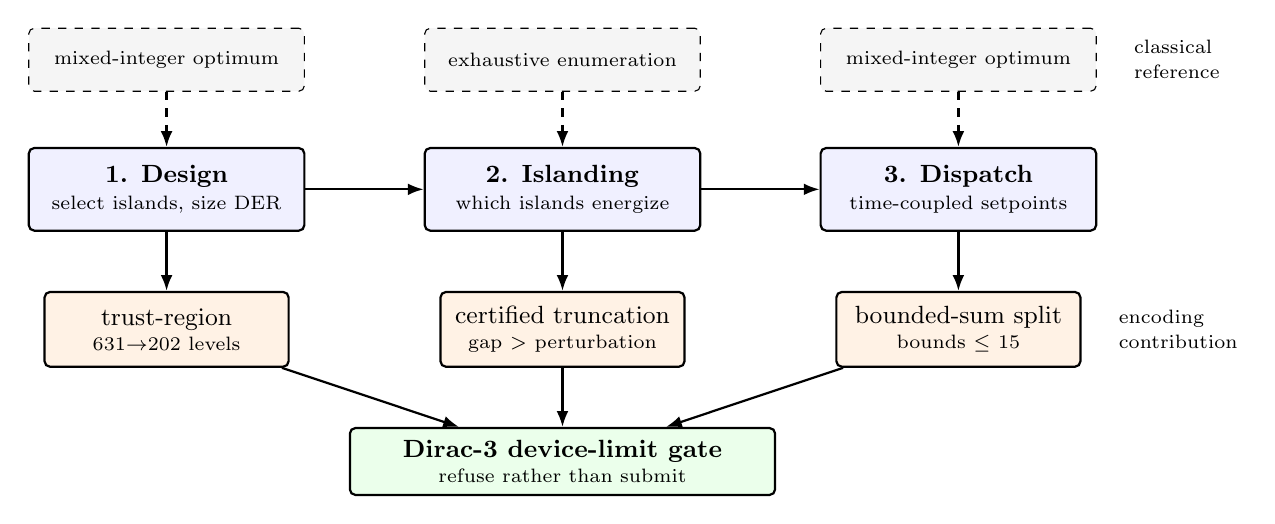
\begin{tikzpicture}[
  font=\small,
  stage/.style={draw,rounded corners=2pt,minimum width=3.5cm,minimum height=1.05cm,
                align=center,fill=blue!6,thick},
  guard/.style={draw,rounded corners=2pt,minimum width=3.1cm,minimum height=0.95cm,
                align=center,fill=orange!10,thick},
  ref/.style={draw,dashed,rounded corners=2pt,minimum width=3.5cm,minimum height=0.8cm,
              align=center,fill=gray!8},
  ar/.style={-{Latex[length=2mm]},thick}]

\node[stage] (d) {\textbf{1. Design}\\[-1pt]{\scriptsize select islands, size DER}};
\node[stage,right=1.5cm of d] (i) {\textbf{2. Islanding}\\[-1pt]{\scriptsize which islands energize}};
\node[stage,right=1.5cm of i] (p) {\textbf{3. Dispatch}\\[-1pt]{\scriptsize time-coupled setpoints}};

\node[guard,below=0.75cm of d] (gd) {trust-region\\[-2pt]{\scriptsize 631$\to$202 levels}};
\node[guard,below=0.75cm of i] (gi) {certified truncation\\[-2pt]{\scriptsize gap $>$ perturbation}};
\node[guard,below=0.75cm of p] (gp) {bounded-sum split\\[-2pt]{\scriptsize bounds $\le$ 15}};

\node[ref,above=0.7cm of d] (rd) {\scriptsize mixed-integer optimum};
\node[ref,above=0.7cm of i] (ri) {\scriptsize exhaustive enumeration};
\node[ref,above=0.7cm of p] (rp) {\scriptsize mixed-integer optimum};

\node[draw,thick,rounded corners=2pt,fill=green!8,below=0.75cm of gi,
      minimum width=5.4cm,minimum height=0.85cm,align=center] (dev)
      {\textbf{Dirac-3 device-limit gate}\\[-2pt]{\scriptsize refuse rather than submit}};

\draw[ar] (d) -- (i);  \draw[ar] (i) -- (p);
\draw[ar] (d) -- (gd); \draw[ar] (i) -- (gi); \draw[ar] (p) -- (gp);
\draw[ar] (gd) -- (dev); \draw[ar] (gi) -- (dev); \draw[ar] (gp) -- (dev);
\draw[ar,dashed] (rd) -- (d); \draw[ar,dashed] (ri) -- (i); \draw[ar,dashed] (rp) -- (p);
\node[right=0.35cm of rp,align=left] {\scriptsize classical\\[-2pt]\scriptsize reference};
\node[right=0.35cm of gp,align=left] {\scriptsize encoding\\[-2pt]\scriptsize contribution};
\end{tikzpicture}
\caption{The three-stage pipeline. Each stage is a bounded-integer polynomial
Hamiltonian (solid boxes), is reduced to within the device's limits by one
encoding contribution (orange), and is measured against an exact classical
method on the identical problem instance (dashed). The device-limit gate
refuses an out-of-range Hamiltonian rather than submitting it, because the
hardware answers such a problem incorrectly without reporting an error.}
\label{fig:pipeline}
\end{figure*}
\section{Technical approach to quantum integration}
\subsection{Certified coefficient truncation}
Write $H(x)=\sum_t c_t \prod_{i \in S_t} x_i$ over integer boxes $x_i \in [0,u_i]$. Partition terms at a floor $c_{\max}/R$ into kept $K$ and dropped $D$. Because every variable is non-negative, the dropped part ranges over an interval $[m_D, M_D]$ we compute exactly, with $\Delta=\sum_{t \in D}|c_t|\prod u_i$. Let $E_1$ be the minimum of $H_K$ and $E_2$ its second-best distinct energy. If $E_2-E_1 > M_D-m_D$, then for any $y$ outside $\arg\min H_K$ we have $H(y) \ge E_2+m_D > E_1+M_D \ge H(x^\star)$, so truncation cannot move the ground state.

Two refinements proved necessary. First, degeneracy: the bound places $\arg\min H$ {\em inside} $\arg\min H_K$, which certifies a unique ground state only when $H_K$ has one minimiser. On all 13 islanding instances where truncation fires, the dropped terms are exactly the per-island switching costs that separate energizing a useful island from energizing a worthless one, so the kept part is degenerate while its gap to the second-best {\em distinct} energy looks large. The bare condition reports success on all of them; requiring uniqueness correctly refuses. Second, the trigger: applying the nominal 23~dB reading would rewrite precisely the 5 highest-range instances of our hardware run --- the strongest evidence we hold --- so we calibrate the trigger to 35~dB, above the 30.9~dB at which the device is {\em observed} resolving correctly. Truncation is default-on and rewrote 0 of 52 Hamiltonians.

\subsection{Trust-region encoding for the design stage}
The design range is intrinsic to encoding {\em absolute} capacity: $c_{\max}$ is the gated offset $\lambda(D/C)^2$ and $c_{\min}$ the photovoltaic square term, so the ratio is $(D_{\max}/12.5)^2 \approx 1.99\times 10^4$ when one unit is 141 times smaller than the largest island demand. Rescaling cannot remove it: normalising per island by $D_c$ measured {\em worse} (42.8 to 59.9~dB), because island demands span 20--1764~kW and the spread merely moves between term families. We instead write $n_{ck} = b_{ck} + d_{ck}$ with $b$ a classical seed and $d$ a bounded correction --- an exact affine substitution. The offset becomes the seed's small residual and bounds shrink to about twice the radius, giving 202 levels, maximum bound 6, and 34.5~dB with the cost ratio unchanged at 1.019$\times$.

\subsection{Bounded-sum decomposition for dispatch}
Base-16 positional digits over-represent: a bound of 40 becomes digits spanning 0--47, so infeasible points are reachable and get clipped, and the $16^k$ weights inflate the range. Measured against the dispatch mixed-integer reference, radix costs 1.640$\times$ at 39.8~dB against 1.060$\times$ at 31.1~dB for splitting each variable into parts whose bounds {\em sum} to exactly $u$. The representable set is then precisely $[0,u]$, clipping cannot occur, and unit weights leave coefficients untouched.

\section{Stakeholder relevance}
Distribution utilities and grid operators plan reinforcements against contingencies they cannot enumerate. Our output is directly actionable for that audience: a minimum-cost build plan, a per-contingency islanding decision, and a dispatch schedule, each with a stated distance from a provable optimum. The capital plan costs 1.019$\times$ a certified mixed-integer optimum on the identical instance, so a planner knows the gap rather than trusting a heuristic.

Three properties matter operationally. Service is supply-capped: no island-hour is credited with more load than its generation supports. Every energized island-hour is validated for voltage and thermal limits after the fact --- 328/331 pass, with the 3 failures thermal rather than voltage, reaching 128\% of line rating. And critical infrastructure is protected structurally: the voltage penalty is capped at an island's non-critical reward, so voltage risk can never strand a hospital or pumping station. Grid-connected operation is also modelled, cutting daily energy cost 29.9\% through storage arbitrage under time-of-use prices.

All network data are publicly released IEEE and MATPOWER test feeders; no proprietary or utility-sensitive data is used.

\section{Results, findings and observations}
\begin{table}[t]\centering\small
\caption{Resilience metrics on the 69-bus feeder over 50
contingency scenarios at seed 42. The reference column is the same grid with no
microgrids, which measures the resilience gained, not a competing algorithm.}
\label{tab:metrics}
\begin{tabular}{@{}lrr@{}}\toprule
Metric & No microgrids & eQoSystem\\\midrule
Worst-hour customers unserved & 100.0\% & \textbf{23.6\%}\\
Critical bus-hours unserved & 397 & \textbf{0}\\
Unserved energy per event (kWh) & 5292 & \textbf{488}\\
Upgrade cost ($\times$10 k\$) & --- & 338.8\\
\bottomrule\end{tabular}\end{table}

\begin{table}[t]\centering\small
\caption{Every stage measured against an exact classical method on the identical
problem instance. Ratios above one are gaps to a proven optimum.}
\label{tab:baselines}
\begin{tabular}{@{}llr@{}}\toprule
Stage & Classical reference & Result\\\midrule
Design & Mixed-integer optimum & 1.019$\times$\\
Islanding & Exhaustive enumeration & 50/50 exact\\
Islanding & Mixed-integer certificate & 50/50 agree\\
Dispatch & Mixed-integer optimum & 0.987$\times$ shed\\
Dispatch & \quad at fuel cost & 1.036$\times$ diesel\\
\bottomrule\end{tabular}\end{table}

\begin{table}[t]\centering\small
\caption{Quantum resource accounting per stage, after the encoding
contributions. Levels are the device's variable-resolution budget, capped at 954
per job; no variable may exceed 16 levels on the integer solver. Dispatch is
shown in the hardware profile, which drops the diesel cubic and splits variables
into bounded parts.}
\label{tab:resources}
\begin{tabular}{@{}lrrrrl@{}}\toprule
Stage & Vars & Levels & Max bd. & dB & Legal\\\midrule
Design & 50 & 202 & 6 & 34.5 & yes\\
Islanding (each) & 3 & 6 & 1 & 0.0--31.1 & yes\\
Dispatch (each) & 37 & 321 & 15 & 31.1 & yes\\
\quad before encoding & 24 & 289 & 43 & 65.0 & no\\
Grid-connected & 36 & 1083 & --- & --- & no\\
\midrule
\multicolumn{6}{@{}l@{}}{\footnotesize 51 jobs per run; design uses 50 integer variables against 104 binary equivalents; 95~s classical wall-clock.}\\
\bottomrule\end{tabular}\end{table}

\subsection{Hardware results}
On Dirac-3, 20/20 islanding instances returned the certified global optimum, with hardware energy equal to the enumeration energy on every one. We disclose that 9 of 20 required active islanding; the remainder were trivial, with ``do nothing'' optimal. Coefficient ranges spanned 0--30.9~dB, and 5 instances exceeded the 23~dB nominal specification (26.1, 29.2, 29.4, 30.7, 30.9~dB) while still resolving correctly --- consistent with the 30.78~dB operating point reported for Dirac-3 elsewhere \citep{space2025}.

The design stage has since also executed on the device, at 34.5~dB and 202 levels for 19~s of billed allocation. It returned a cheaper but less feasible raw solution than the classical annealer (324.8 against 329.8), needing 6 feasibility repairs against three and finishing at 1.064$\times$ the certified optimum. We report that as a measured hardware quality gap, not parity. It does establish that the device resolves a 34.5~dB Hamiltonian, which is direct evidence for the calibrated trigger over the datasheet figure.

\subsection{Negative and null results}
{\em Voltage awareness changes nothing here.} We encode predicted worst-bus voltage as a degree-1 penalty, and both arms are identical on every metric because the penalty is identically zero: the worst predicted voltage across all candidates is 0.9904~pu against a 0.95~pu band. Islands are electrically short and fed from generation sited inside them. The binding physical constraint is thermal, not voltage.

{\em The design gap is a formulation limit, not solver budget.} The cost ratio is flat across the effort sweep, and annealing finds {\em lower} Hamiltonian energy than its own warm start while decoding to {\em higher} post-repair cost. Reweighting does not help either: repricing the slack variable and raising the capacity weight tenfold both leave the ratio unmoved. The penalty objective is not the reported metric, and closing that needs hard constraints the penalty form structurally lacks.

{\em Stochastic value is real but assumption-dependent.} With lost load at \$10/kWh, the value of the stochastic solution is 0.22 and of perfect information 3.85 (annualised, $\times$10 k\$). Across plausible outage costs and event rates the optimal sizing margin moves and the stochastic value vanishes when outages are cheap. The design Hamiltonian is scenario-independent, so what is studied here is the sizing margin, not a fully scenario-coupled program.

{\em Cross-island export works and is deliberately not enabled.} Rewarding tie-connected island pairs cuts unserved energy 488 to 264~kWh, serving 65 bus-instances no single island can reach. It changes the islanding Hamiltonian, which would make our recorded hardware energies unreproducible from the submitted code, so it ships as a reported arm rather than a silent default.

\section{Conclusions}
Certified coefficient truncation and trust-region encoding together move a three-stage microgrid planning pipeline inside the limits of an entropy quantum computer, and they do it with proofs rather than assurances. Truncation rewrites a Hamiltonian only when a spectral-gap certificate holds and a uniqueness check passes, and its trigger is set by what the hardware is observed to resolve rather than by a datasheet. The trust-region encoding reaches 202 levels and 34.5~dB with the cost ratio unchanged, and bounded-sum decomposition brings dispatch within every device limit while base-16 decomposition does not.

The resilience outcome is a worst-hour unserved fraction of 23.6\% and 0 critical bus-hours lost against a 397 bus-hour reference, at a capital plan 1.019$\times$ a certified optimum, with 20/20 islanding instances and the design stage executed on real hardware. We claim no speedup: at this scale exact classical methods are fast and we say so. What the device buys is representational --- integer variables and degree-3 gating without auxiliaries, at 2.1$\times$ fewer variables than binary compilation.

Three doors stand open. Cross-island export is built and measured and needs only a short hardware re-run to adopt. The exact mixed-integer certifier we introduce proves optima at 40 binary variables in seconds, where enumeration would need $10^{12}$ states, so certification no longer limits growth of the candidate pool. And because islanding problem size scales with candidate count rather than bus count, a feeder of several thousand buses reduced to a few dozen candidates remains a single job well inside the device's budget.

\balance
\onecolumn
\begin{thebibliography}{9}\small
\bibitem{nguyen2024} N.~T.~M. Nguyen et al., ``Entropy computing: a paradigm for
optimization in open photonic systems,'' arXiv:2407.04512, 2024.
\bibitem{space2025} Dirac-3 application to space logistics planning,
arXiv:2501.05046, 2025.
\bibitem{baranwu1989} M.~E. Baran and F.~F. Wu, ``Network reconfiguration in
distribution systems for loss reduction and load balancing,''
\textit{IEEE Trans. Power Delivery}, vol.~4, no.~2, pp.~1401--1407, 1989.
\bibitem{nikmehr2024} N.~Nikmehr et al., ``Quantum annealing-infused microgrids
formation,'' \textit{IEEE Trans. Power Systems}, 2024.
\bibitem{qmgf2024} ``Reforming quantum microgrid formation,'' arXiv:2406.05916, 2024.
\bibitem{chenvu2025} Y.~Chen and T.~L. Vu, ``A review of quantum computing
technologies in power system optimization,'' PNNL-37598, 2025.
\bibitem{critical2026} ``A critical comment on entropy computing,''
arXiv:2605.03612, 2026.
\bibitem{glover1974} F.~Glover and E.~Woolsey, ``Converting the 0-1 polynomial
programming problem to a 0-1 linear program,'' \textit{Operations Research},
vol.~22, no.~1, pp.~180--182, 1974.
\bibitem{morstyn2024} T.~Morstyn and X.~Wang, ``Opportunities for quantum
computing within net-zero power system optimization,'' \textit{Joule}, vol.~8,
no.~6, pp.~1619--1640, 2024.
\end{thebibliography}
\end{document}
